\subsection{Discussion}
%
In order to analyze the measurements the signal as well as the noise are loaded and fourier transformed. In the next step the noise is substracted from the signal in order to reduce the noise in the actual measurement.\enlargethispage{\baselineskip}\p
To display the beamforming characteristics of different AM and FM signals the amplitude of the corresponding frequency is picked from the frequency spectrum. This is done for every angle. In the end the power of the signal in relation to the highest value is calculated in $dB$. Figures \ref{fig:meas:beam:polar_meas_am} and \ref{fig:meas:beam:polar_meas_am} show the resulting characteristics.\p
For comparison a graph using the same number of transducers ($5$) and the same distance between them ($10.5mm$) as the real speaker was created using the results from section \secref{sec:theory:beam}. It is displayed in figure \ref{fig:meas:beam:polar_calc}.
%
\begin{figure}
  \centering
  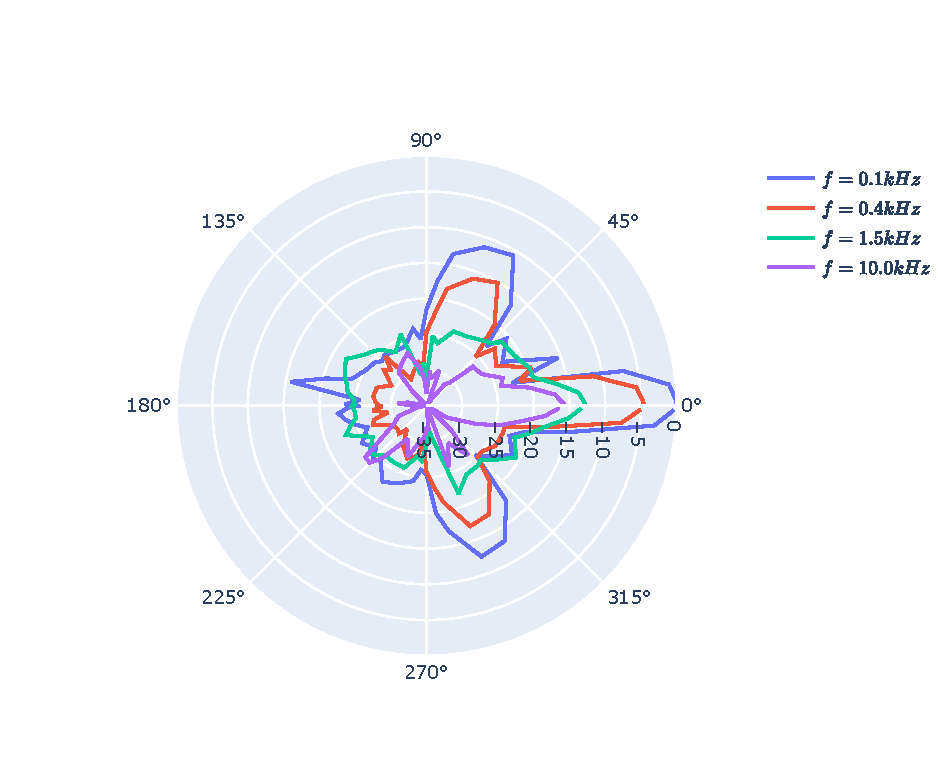
\includegraphics[height=\largeheight]{src/assets/pictures/measurements/beamforming_am_polar.pdf}
  \caption{Measured beamforming characteristics of AM signals}\label{fig:meas:beam:polar_meas_am}
\end{figure}
%
\begin{figure}
  \centering
  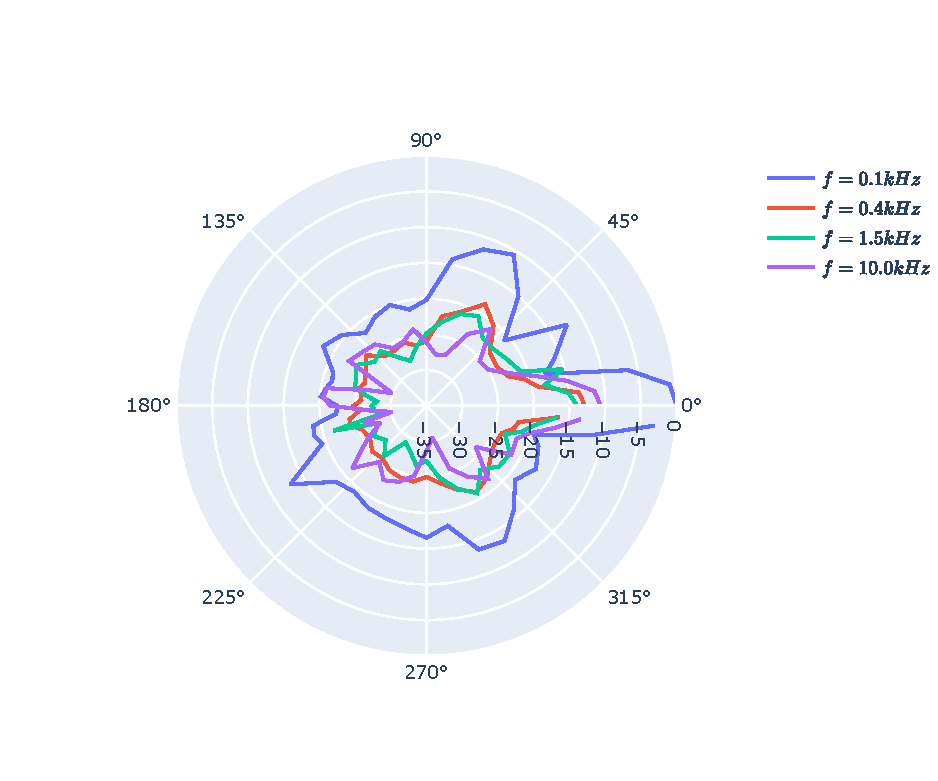
\includegraphics[height=\largeheight]{src/assets/pictures/measurements/beamforming_fm_polar.pdf}
  \caption{Measured beamforming characteristics of FM signals}\label{fig:meas:beam:polar_meas_fm}
\end{figure}
\p
% side lobes
Both AM and FM signals show clear beamforming behaviour. Having said this the signal amplitude outside of the beam seems to be much higher for FM signals. Additionally, two side lobes at around $\pm 65^\circ$ can be observed. They arise because the distance between the transducers is significantly higher than $\frac{\lambda}{2}$ and can also be seen in figure \ref{fig:meas:beam:polar_calc}. While analyzing the results for all measured frequencies it was noticed that the power of the signal as well as the beamforming effect was smallest for signals between $1kHz$ and $2kHz$.
%
\begin{figure}
  \centering
  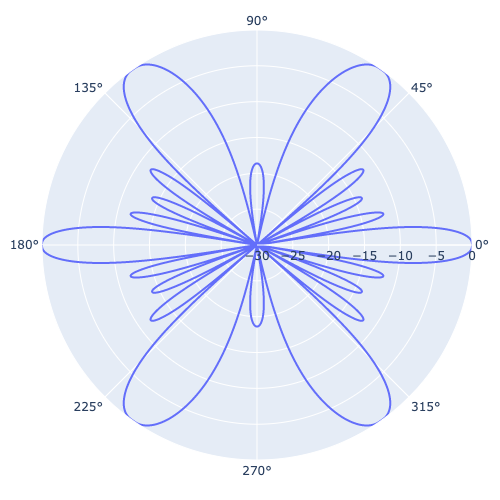
\includegraphics[height=\mediumheight]{src/assets/pictures/measurements/beamforming_calc_polar.png}
  \caption{Calculated beamforming characteristics}\label{fig:meas:beam:polar_calc}
\end{figure}